% =====================================================================
% 3. Fundamentação teórica
% =====================================================================
\section{Fundamentação teórica}
\label{sec:teoria}

\subsection{Problema de valor inicial}

Seja \(y(t)\in\mathbb{R}^{m}\) a solução de
\begin{equation}
y'(t) = f(t,y(t)), \qquad y(t_0)=y_0.
\label{eq:pvi}
\end{equation}
Se \(f\) é contínua e lipschitziana em \(y\), numa faixa que contém a solução, o problema de valor inicial tem solução única \cite{boyce2012,hairer1993}. Um método de passo único produz \(y_{n+1}\) usando apenas \(t_n\), \(y_n\) e o passo \(h_n\). A consistência de ordem \(p\) significa que o erro local de truncamento, cometido num único passo a partir do valor exato, é \(\mathcal{O}(h^{p+1})\). Se o método também é zero-estável, o erro global num intervalo fixo \([t_0,t_f]\) é \(\mathcal{O}(h^{p})\) quando \(h\to 0\) \cite{hairer1993,quarteroni2007}.

A zero-estabilidade é uma propriedade do método no limite de passo nulo: perturbações pequenas não podem ser amplificadas de forma ilimitada quando o número de passos cresce e \(h\) diminui. Os métodos explícitos de Runge-Kutta usados aqui são zero-estáveis. Isso não impede que, para um \(h\) fixo e positivo, a iteração amplifique o modo próprio do sistema. Essa segunda propriedade é a estabilidade absoluta, tratada na Seção~\ref{sec:estabilidade}. Confundi-las leva a concluir, erroneamente, que um método convergente pode usar qualquer passo.

\subsection{O circuito RLC série}
\label{sec:modelo}

A Figura~\ref{fig:circuito} mostra o circuito. A lei das tensões de Kirchhoff no laço e a lei do capacitor dão
\begin{equation}
L\frac{di}{dt}+Ri+v_C = v_s(t), \qquad C\frac{dv_C}{dt}=i.
\label{eq:kvl}
\end{equation}
Com o estado \(y=[i,\;v_C]^{\mathsf T}\),
\begin{equation}
f(t,y)=
\begin{bmatrix}
\bigl(v_s(t)-Ri-v_C\bigr)/L \\
i/C
\end{bmatrix}.
\label{eq:sistema}
\end{equation}
Essa descrição de estados é a forma usual do RLC série em análise de circuitos \cite{nilsson2019}. A matriz do sistema homogêneo é
\begin{equation}
A=
\begin{bmatrix}
-R/L & -1/L \\
1/C & 0
\end{bmatrix}.
\label{eq:matriz}
\end{equation}
Os autovalores satisfazem \(\lambda^{2}+2\alpha\lambda+\omega_0^{2}=0\), com amortecimento \(\alpha=R/(2L)\) e pulsação natural \(\omega_0=1/\sqrt{LC}\). O fator de qualidade do série é \(Q=\omega_0 L/R=1/(2\zeta)\), em que \(\zeta=\alpha/\omega_0\).

\begin{figure}[htbp]
\centering
\caption{Circuito RLC série usado como protótipo do estágio ressonante. A fonte \(v_s(t)\) é um degrau, uma senoide ou um pulso.}
\label{fig:circuito}
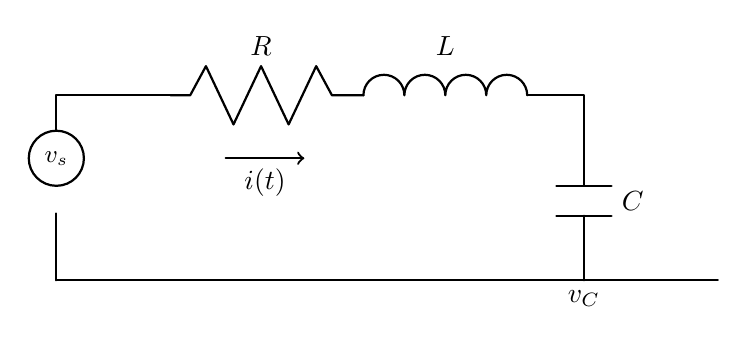
\begin{tikzpicture}[thick,line cap=round,line join=round]
  \draw (0,0) -- (8.4,0);
  \draw (0,0) -- (0,0.85);
  \draw (0,1.55) circle (0.35);
  \node at (0,1.55) {\small $v_s$};
  \draw (0,1.90) -- (0,2.35) -- (1.45,2.35);
  \draw (1.45,2.35) -- (1.70,2.35) -- (1.90,2.72) -- (2.25,1.98) -- (2.60,2.72)
        -- (2.95,1.98) -- (3.30,2.72) -- (3.50,2.35) -- (3.90,2.35);
  \node[above] at (2.60,2.72) {$R$};
  \draw (3.90,2.35) arc (180:0:0.26) arc (180:0:0.26) arc (180:0:0.26) arc (180:0:0.26);
  \node[above] at (4.94,2.72) {$L$};
  \draw (5.98,2.35) -- (6.70,2.35) -- (6.70,1.20);
  \draw (6.35,1.20) -- (7.05,1.20);
  \draw (6.35,0.82) -- (7.05,0.82);
  \node[right] at (7.05,1.01) {$C$};
  \draw (6.70,0.82) -- (6.70,0);
  \draw[->] (2.15,1.55) -- (3.15,1.55) node[midway,below] {$i(t)$};
  \node[below] at (6.70,0) {$v_C$};
\end{tikzpicture}
\fonte{Elaborado pelo autor (2026).}
\end{figure}

O discriminante \(\alpha^{2}-\omega_0^{2}\) separa os regimes. Se \(\alpha<\omega_0\), a resposta livre oscila com \(\omega_d=\sqrt{\omega_0^{2}-\alpha^{2}}\). Se \(\alpha=\omega_0\), o amortecimento é crítico. Se \(\alpha>\omega_0\), há dois polos reais, \(\lambda=-\alpha\pm\beta\), com \(\beta=\sqrt{\alpha^{2}-\omega_0^{2}}\).

Para \(v_s(t)=V_0\) constante e condições iniciais nulas, a corrente e a tensão no capacitor são, no regime subamortecido,
\begin{align}
i(t)&=\frac{V_0}{\omega_d L}e^{-\alpha t}\sin(\omega_d t), \label{eq:i-sub}\\
v_C(t)&=V_0\left[1-e^{-\alpha t}\left(\cos(\omega_d t)+\frac{\alpha}{\omega_d}\sin(\omega_d t)\right)\right]. \label{eq:vc-sub}
\end{align}
No caso crítico, \(i(t)=(V_0/L)\,t\,e^{-\alpha t}\) e \(v_C(t)=V_0\bigl[1-e^{-\alpha t}(1+\alpha t)\bigr]\). No caso sobreamortecido,
\begin{equation}
i(t)=\frac{V_0}{\beta L}e^{-\alpha t}\sinh(\beta t).
\label{eq:i-sobre}
\end{equation}
A tensão correspondente troca seno e cosseno por seno e cosseno hiperbólicos. Essas expressões foram conferidas pela lei de Kirchhoff com a derivada analítica da corrente: o resíduo máximo ficou na ordem de \(10^{-15}\)~V, isto é, no arredondamento de máquina.

Para \(v_s(t)=V_m\sin(\omega t)\) e condições iniciais nulas, a corrente permanente tem amplitude \(V_m/|Z|\), com \(Z=R+j\bigl(\omega L-1/(\omega C)\bigr)\), e fase igual ao oposto do argumento de \(Z\). Na ressonância, \(\omega=\omega_0\), \(Z=R\) e a solução completa é
\begin{equation}
i(t)=\frac{V_m}{R}\left[\sin(\omega_0 t)-\frac{\omega_0}{\omega_d}e^{-\alpha t}\sin(\omega_d t)\right].
\label{eq:i-res}
\end{equation}
Fora da ressonância, a solução particular \(D\cos(\omega t)+E\sin(\omega t)\) foi obtida pelo sistema linear proveniente da equação diferencial da corrente, e as constantes da solução homogênea foram fixadas pelas condições iniciais. O resíduo da equação diferencial, com derivadas analíticas, ficou na ordem de \(10^{-10}\)~A/s. A tensão no capacitor segue de \(v_C=v_s-Ri-L\,di/dt\).

\subsection{Euler e Euler melhorado}

O método de Euler avança pela reta tangente,
\begin{equation}
y_{n+1}=y_n+h f(t_n,y_n).
\label{eq:euler}
\end{equation}
A série de Taylor da solução exata é \(y(t_n+h)=y+hf+\frac{h^{2}}{2}y''+\mathcal{O}(h^{3})\). O método retém os dois primeiros termos. O erro local é \(\frac{h^{2}}{2}y''(\xi)\), e o erro global num intervalo fixo é \(\mathcal{O}(h)\), desde que o passo esteja na região de estabilidade \cite{burden2016,chapra2015}.

O Euler melhorado, ou método de Heun, usa a média entre a derivada no início do passo e a derivada prevista no fim:
\begin{align}
k_1&=f(t_n,y_n), \nonumber\\
k_2&=f(t_n+h,\,y_n+hk_1), \nonumber\\
y_{n+1}&=y_n+\frac{h}{2}(k_1+k_2). \label{eq:heun}
\end{align}
Expandindo \(k_2=f+h y''+\mathcal{O}(h^{2})\) e substituindo, o incremento reproduz Taylor até \(\frac{h^{2}}{2}y''\). O erro local passa a \(\mathcal{O}(h^{3})\) e o erro global a \(\mathcal{O}(h^{2})\) \cite{heun1900,hairer1993}. O método de Euler modificado, ou do ponto médio, é outro Runge-Kutta de ordem 2, com a avaliação no meio do passo. Para sistemas lineares, os dois têm a mesma função de estabilidade \(R(z)=1+z+z^{2}/2\), porque o polinômio de grau 2 que copia a exponencial até a ordem 2 é único. As constantes de erro, porém, diferem. O código implementa o Euler melhorado, que é a forma pedida pela disciplina.

\subsection{Runge-Kutta clássico de quarta ordem}

O método clássico avalia a função quatro vezes:
\begin{align}
k_1&=f(t_n,y_n), \nonumber\\
k_2&=f\!\left(t_n+\frac{h}{2},\,y_n+\frac{h}{2}k_1\right), \nonumber\\
k_3&=f\!\left(t_n+\frac{h}{2},\,y_n+\frac{h}{2}k_2\right), \nonumber\\
k_4&=f(t_n+h,\,y_n+hk_3), \nonumber\\
y_{n+1}&=y_n+\frac{h}{6}(k_1+2k_2+2k_3+k_4). \label{eq:rk4}
\end{align}
O quadro de Butcher correspondente é
\begin{equation}
\begin{array}{c|cccc}
0\\
1/2 & 1/2\\
1/2 & 0 & 1/2\\
1 & 0 & 0 & 1\\
\hline
& 1/6 & 1/3 & 1/3 & 1/6
\end{array}
\label{eq:butcher}
\end{equation}
Os coeficientes satisfazem as condições de ordem até 4. O erro local é \(\mathcal{O}(h^{5})\) e o erro global é \(\mathcal{O}(h^{4})\) enquanto a solução for suficientemente suave e o passo, estável \cite{kutta1901,butcher2016,hairer1993}. Cada passo custa quatro avaliações de \(f\). A comparação justa de custo não é o número de passos, e sim o número de avaliações necessário para um erro prescrito.

\subsection{Estabilidade absoluta}
\label{sec:estabilidade}

Aplicado à equação de teste \(y'=\lambda y\), um Runge-Kutta explícito produz \(y_{n+1}=R(h\lambda)y_n\). A região de estabilidade absoluta é o conjunto dos \(z\in\mathbb{C}\) com \(|R(z)|\le 1\). Para o Euler, \(R(z)=1+z\). Para o Heun, \(R(z)=1+z+z^{2}/2\). Para o RK4,
\begin{equation}
R(z)=1+z+\frac{z^{2}}{2}+\frac{z^{3}}{6}+\frac{z^{4}}{24}.
\label{eq:Rrk4}
\end{equation}
No circuito, \(\lambda\) são os dois autovalores de \(A\). O passo é estável se ambos caem dentro da região.

No regime subamortecido, \(\lambda=-\alpha\pm j\omega_d\). Para o Euler, \(|1+h\lambda|\le 1\) simplifica-se para
\begin{equation}
0<h\le\frac{2\alpha}{\omega_0^{2}}=RC=\frac{1}{\omega_0 Q}.
\label{eq:heuler}
\end{equation}
O limite depende do fator de qualidade. Um tanque seletivo, de \(Q\) alto, empurra o Euler para passos muito menores do que o período da oscilação. Na fronteira, \(|R|=1\): o modo não explode, mas o amortecimento numérico já não é o amortecimento do circuito. Acima da fronteira, \(|R|>1\) e o erro cresce a cada passo. Perto da fronteira o crescimento é lento; longe dela, a solução estoura em poucos períodos.

Para polos reais negativos, a condição \(|1+h\lambda|\le 1\) equivale a \(h\le 2/|\lambda|\). O polo de maior módulo é o mais exigente. A fórmula \(h\le RC\) não deve ser reutilizada fora do regime subamortecido.

O RK4 inclui um trecho do eixo imaginário até \(|\mathrm{Im}(z)|\approx 2\sqrt{2}\approx 2{,}83\). Num circuito de \(Q\) alto, \(|\lambda|\approx\omega_0\), e o passo estável chega à ordem de \(2{,}8/\omega_0\), quase independente de \(Q\). Essa diferença, e não apenas a ordem, é o motivo prático para preferir o RK4 na simulação de filtros seletivos. Os limites do Heun e do RK4 para os parâmetros deste estudo foram calculados varrendo \(h\) até \(|R(h\lambda)|\) ultrapassar 1, e conferidos pela integração.

\subsection{Arredondamento}

O erro global observado é a soma do erro de truncamento, que cai como \(h^{p}\), e do erro de arredondamento, que não obedece à mesma lei. Em precisão dupla, o segundo só aparece com passos muito pequenos ou com muitas operações. Em precisão simples, o piso surge cedo. Reduzir \(h\) além desse piso piora o resultado, porque aumentam as operações sem ganho de truncamento \cite{goldberg1991,higham2002}. O controlador de passo e a escolha do formato precisam ser decididos juntos: uma tolerância de \(10^{-12}\) não é atingível em \emph{binary32} neste problema, qualquer que seja o passo.

\subsection{Passo adaptativo}

No problema linear de coeficientes constantes, o melhor passo fixo é quase constante, porque a escala de tempo não muda. Um controlador ainda é útil quando a excitação tem trechos mortos e trechos rápidos, e é o mecanismo que transforma uma tolerância pedida pelo usuário num passo. O código usa duplicação de passo \cite{press2007,hairer1993}. Um passo de tamanho \(h\) é comparado com dois passos de tamanho \(h/2\). Para um método de ordem 4, o erro local escala com \(h^{5}\), e dois meios passos acumulam \(2\times(h/2)^{5}=h^{5}/16\). A diferença \(\Delta\) entre as duas soluções estima \(\frac{15}{16}\) do erro local do passo cheio. O erro da solução de dois meios passos, que é a aceita, é estimado por \(\|\Delta\|/15\).

A norma é relativa e absoluta, componente a componente:
\begin{equation}
\mathrm{err}=\frac{1}{15}\max_i\frac{|\Delta_i|}{\mathrm{atol}+\mathrm{rtol}\,|y_i|}.
\label{eq:erradap}
\end{equation}
O passo é aceito se \(\mathrm{err}\le 1\). O passo seguinte é
\begin{equation}
h_{\mathrm{novo}}=h\cdot\min\bigl(2,\;\max(0{,}2,\;0{,}9\,\mathrm{err}^{-1/5})\bigr).
\label{eq:hnovo}
\end{equation}
Há um teto de tentativas, para que uma tolerância impossível não produza um laço sem fim. O erro global não coincide com a tolerância local: ele acumula ao longo do intervalo. A tolerância é um controle do passo, não uma garantia direta sobre \(y(t_f)\).
